\documentclass{article}		
\usepackage{amsmath}
\usepackage{bbm}
\usepackage{amsthm}
\usepackage{amssymb}
\usepackage{graphicx}
\usepackage{prodint}
\usepackage[margin=0.2cm,footskip=0.25cm]{geometry}
\usepackage[swedish,english]{babel}
\setlength{\parindent}{0pt}

\title{Cheat Sheet}
\author{Anton Stråhle \& Jan Alexandersson}

\begin{document}

\section*{Nelson-Aalen \& Kaplan-Meier}

\textbf{Basic Relations}

$S(t) = \exp(-\int_0^t \alpha(s)ds) \qquad A(t) = \int_0^t \alpha(s)ds \qquad -S'(t) = \alpha(t)S(t) \qquad f(t)=\alpha(t) S(t) \qquad P(T>x | T>y) = \frac{P(T>x)}{P(T>y)} = \frac{S(x)}{S(y)} \\ \lambda(s) = \alpha(s)Y(s)$ 

\medskip

\textbf{Nelson-Aalen} Non-parametric estimator of the cumulative hazard rate. $A(t) = \int_0^t \alpha(u) du$ where $\alpha(t)$ is the hazard rate at time $t$. 

\medskip

\textbf{Formulas} $ \hat{A}(t) = \sum_{T_j \leq t} \Delta \hat{A}(T_j)$ \newline
$
\text{No ties } \Delta \hat{A}(T_j) = \frac{1}{Y(T_j)} \quad
\text{Rounded Ties } \Delta \hat{A}(T_j) = \sum_{k=1}^{d_j -1}\frac{1}{Y(T_j) - k} \quad
\text{True Ties } \Delta \hat{A}(T_j) = \frac{d_j}{Y(T_j)} $ \newline $
\hat\sigma^2_{\text{N-A}}(t) = \sum_{T_j \leq t} \Delta \hat\sigma^2(T_j) $\newline 
$
\text{No ties } \Delta \hat\sigma^2(T_j) = \frac{1}{Y(T_j)^2} \quad
\text{Rounded Ties } \Delta \hat\sigma^2(T_j) = \sum_{k=1}^{d_j -1}\frac{1}{(Y(T_j) - k)^2} \quad
\text{True Ties } \Delta \hat\sigma^2(T_j) = \frac{(Y(T_j)-d_j)d_j}{Y(T_j)^3}$

\medskip


\textbf{Derivation of the Nelson-Aalen Estimator}. $M(t)$ is a mean-zero m.g. $H(t) = \frac{J(t)}{Y(t)}$ is predictable where $J(t) = \mathbf{1}(Y(t) > 0)$. We then get $\hat{A}(t) = \int_0^t H(s)dN(s) = \int_0^t\alpha(s)J(s)ds + \int_0^t \frac{J(s)}{Y(s)}dM(s)$. As $M(t)$ is mean-zero m.g. we then get that the Nelson-Aalen estimator is a unbiased estimator of $A^*(t) = \int_0^t \alpha(s)J(s)ds $ since $\mathbb{E}\left[\hat{A}(t) - A^*(t)\right] = 0$. $\hat{A}(t)$ is however a biased estimator of $A(t)$ since $\mathbb{E}[J(s)] = \mathbb{P}(Y(s) > 0)$. This bias is however very small.

\medskip


\textbf{Derivation of variance of Nelson-Aalen Estimator}. Recall that $\left[\int HdM\right](t) = \int H(s)^2dN(s)$ where we have $H(s) = \frac{J(s)}{Y(s)} \implies \left[\int HdM\right](t) = \int \left(\frac{J(s)}{Y(s)}\right)^2dN(s) = [\hat{A} - A^*](t) \implies \hat\sigma^2_{\text{N-A}} = \sum_{T_j \leq t} \frac{1}{Y(T_j)}$ 

\medskip


\textbf{Delta Method CI Nelson-Aalen} We have that $\hat{A}(t)\overset{\text{approx}}{\sim} N(A(t), \hat\sigma^2(t))$
\begin{align*}
	g(\hat{A}(t)) &\approx g(A(t)) + g'(A(t))\underbrace{(\hat{A}(t)-A(t))}_{\mathbb{E}[...] = 0}
	\implies \mathbb{E}[g(\hat{A}(t))] \approx g(A(t)) \text{ and } \mathbb{E}[(g(\hat{A}(t))- g(A(t))^2] \approx g'(\hat{A}(t))^2\underbrace{\mathbb{E}[(\hat{A}(t) - A(t))^2]}_{\hat\sigma^2}  \\
	\implies g(\hat{A}(t)) &\overset{\text{approx}}{\sim} N(g(A(t), |g'(\hat{A}(t)|\hat\sigma)
\end{align*}
Let $g(x) = \log(x)$ which then gives us $g^{-1}(x) = e^x$ and $g'(x) = \frac{1}{x}$. The interval then becomes as follows. \newline
$g^{-1}(CI) = \text{exp}\left\{\log(\hat{A}(t)) \pm z_{1-\alpha/2}\frac{\hat\sigma}{\hat{A}(t)}\right\} = \hat{A}(t)\text{exp}\left\{\pm z_{1-\alpha/2}\frac{\hat\sigma}{\hat{A}(t)}\right\}$

\medskip

\textbf{Kaplan-Meier} Non-parametric estimator of the survival function. $S(t) = e^{-A(t)}$ where $A(t)$ is the cumulative hazard rate at time $t$.

\medskip

\textbf{Formulas} $\hat{S}(t) = \prod_{T_j\leq t}\left(1-\frac{1}{Y(T_j)}\right) = \prod_{T_j \leq t} (1- \Delta \hat{A}(T_j))$ \newline
$\hat\tau^2(t) = \hat{S}(t)^2\sum_{T_j \leq t} \frac{1}{Y(T_j)^2} = \hat{S}(t)^2\hat\sigma^2_{\text{N-A}} \quad \hat\tau^2(t) = \hat{S}(t)^2 \sum_{T_j \leq t}\frac{d_j}{Y(T_j)(Y(T_j)-dj)} \text{ (Greenwood)}$

\medskip

\textbf{Derivation of the Kaplan-Meier Estimator} Recall $\mathbb{P}(T > t) \implies S(t_k|t_{k-1}) = \mathbb{P}(T>t_k|T>t_{k-1}) = \frac{S(t_k)}{S(t_{k-1)}}$. Let $0 = t_0 < t_1 < \hdots < t_n$ and note that $\mathbb{P}(T>t_0) = 1$ which gives us $S(t_n) = \prod_{k=1}^n\frac{S(t_k)}{S(t_{k-1})}$. We formally we define the survival function as $S(t) = \prodi_{u\leq t} (1-dA(u))$ since $\frac{S(t_k)}{S(t_{k-1})} = dA(t_k)$ when $t_k - t_{k-1} <<1$. This gives us the estimator $\hat{S}(t) = \prod_{T_j \leq t} (1-\Delta \hat{A}(T_J))$ as $\Delta \hat{A}(t)$ serves as an estimator for $dA(t)$. 

\medskip


\textbf{Kaplan Meier CI} $\hat{S}(t) \pm z_{1-\alpha/2}\hat{\tau}(t)$. Log-transforms (using same method as for Nelson-Aalen above) etc. 

\medskip

\textbf{Derivation of variance of Kaplan-Meier Estimator} 
Let $S^*(t) = \prodi_{u\leq t} (1-dA^*(t))$ where $A^*(t) = \int_0^t J(u)dA(u)$. If $\mathbb{P}(J(s) = 0) << 1$ then $S^*$ and $S$ are close. We measure this closeness by $\frac{\hat{S}(t)}{S^*(t)} - 1 = -\int_0^t \frac{\hat{S}(u-)}{S^*(u)}d(\hat{A} - A^*)(u)$. We then have that $\mathbb{E}\left[\frac{\hat{S}(t)}{S^*(t)}\right] = 1$. We can then repeat the arguments as we do for the variance of the Nelson-Aalen estimator above. $\left[\frac{\hat{S}}{S^*} - 1\right] = \left[\int \frac{-\hat{S}}{S^*}\underbrace{d(\hat{A} - A^*)}_{dM}\right] = \{\text{Theorem}\} = \int \left(\frac{\hat{S}}{S^*}\right)^2d[M]$. Note that $M$ is the same mean-zero m.g. as in the Nelson-Aalen case which gives us $d[M](t)=\frac{J(t)}{Y(t)}dN(t)$. This does in turn give us that $\left[\frac{\hat{S}}{S^*}-1\right] = \int \left(\frac{\hat{S}}{S^*}\right)^2 \frac{J}{Y^2}dN$. Now by assuming $S^* = S$ and $\hat{S}(u) \approx \hat{S}(u-)$ we get that $\text{Var}\left(\frac{\hat{S}(t)}{S(t)} - 1\right) = \hat\sigma^2_{\hat{S}/S- 1}(t) = \int_0^t \frac{J}{Y^2}dN = \hat\sigma^2_{\text{N-A}}(t) \implies \hat\sigma^2_{\hat{S}}(t) \approx \hat{S}^2(t)\int_0^t \frac{J}{Y^2}dN = \hat{S}^2(t)\hat\sigma^2_{\text{N-A}}(t)$

\newpage

\section*{Martingales}

\textbf{Definition of Martingales} $M$ is a Martingale if $E[M_t | \mathcal{F}_{s}] = M_s, \quad t\geq s$ and $E[|M_t|] < \infty$. 

\medskip

\textbf{Formulas} 

\begin{minipage}{0.5\textwidth}
	\begin{align*}
		(H\bullet M)_n &= H_0M_0 + H_1(M_1-M_0) + \hdots + H_n(M_n-M_{n-1}) \\
		\langle H\bullet M \rangle_n &= \sum_{i=1}^n H_i^2\Delta\langle M\rangle_i \text{ where }\Delta \langle M\rangle_i = [(M_i - M_{i-1})^2|\mathcal{F}_{i-1}]\\
		\langle H\bullet M\rangle &= H^2\bullet \langle M\rangle \\
		\langle M \rangle_n &= \sum_{i=1}^n \text{Var}(\Delta M_i| \mathcal{F}_{i-1}) = \sum_{i=1}^n \mathbb{E}[(M_i - M_{i-1})^2|\mathcal{F}_{i-1}] \\
		\left\langle \int HdM\right\rangle &= \int H^2(s)d\langle M\rangle(s) = \int H^2(s) \lambda(s)ds \\
		\\
		&Cov(M_s, M_t-M_s) = 0 \\
		&M^2 - \langle M \rangle \text{ and } M^2 - [M] \text{ are zero mean m.g.s. }\\
		&Var (M(t)) = E\Big( M(t) \Big)^2 = E \langle M \rangle (t) = E[M](t)
	\end{align*}
\end{minipage}
\begin{minipage}{0.5\textwidth}
	\begin{align*}
		\Delta M_t &= M_t - M_{t-1} \text{ called m.g. difference}\\
		[H\bullet M]_n &= \sum_{i=1}^n H_i^2\Delta[M]_i \text{ where }\Delta [M]_i = (M_i - M_{i-1})^2\\
		[H\bullet M] &= H^2\bullet[M] \\
		[M]_n &= \sum_{i=1}^n (\Delta M_i)^2 = \sum_{i=1}^n (M_i -M_{i-1})^2 \\
		\left[ \int HdM\right] &= \int H^2(s)d[ M]s) = \int H^2(s) dN(s) \\
		\\
		&E[M_t-M_s | \mathcal{F}_s] = E[M_t|\mathcal{F}_s] - M_s = 0 \\
		&E[\Delta M_t | \mathcal{F}_{t-1}] = 0
	\end{align*}
\end{minipage}

\medskip

\textbf{Doob decomposition}
Let $X$ with $X_0$ be a general discrete time proc. and let $M$ be def. by $M_0 = X_0=0$ and \\  $\underbrace{M_n-M_{n-1}}_{\Delta M_n} = X_n-E[X_n|\mathcal{F}_{n-1}]$
$\implies E[\Delta M_n | \mathcal{F}_{n-1}] = 0 \implies X_n = E[X_n | \mathcal{F}_{n-1}] + \Delta M_n = \underbrace{E[X_n | \mathcal{F}_{n-1}]}_{pred.} + \underbrace{(X_n-E[X_n| \mathcal{F}_{n-1}])}_{noise}$

\newpage

\section*{Frailty}

\textbf{Basic Relations}  $A(t|Z) = \int_0^t \alpha(s|Z)ds$ if proportional frailty (i.e. $\alpha(t|Z) = \alpha(t)Z$ we have $A(t|Z) = ZA(t) \implies S(t) = \text{exp}\{-ZA(t)\}$. Consequently the piopulation survival is given by $S(t) = \mathbb{E}[S(t|Z)] = \mathbb{E}\left[\text{exp}\{-A(t|Z)\}\right] = \mathcal{L}_Z(A(t))$ where $\mathcal{L}_Z(c)$ is the Laplace transform (i.e. $\Psi_Z(-c)$).

\medskip

\textbf{Population Hazard Rate} $\mu(t) = \frac{-S'(t)}{S(t)} = \alpha(t)\frac{\mathcal{L}'(A(t))}{\mathcal{L}(A(t))}$ assuming proportional frailty ($\alpha(t|Z) = \alpha(t)Z$

\medskip 

\textbf{Modelling Frailty as Power Variance Function} We let $Z \sim \text{PVF}(\varphi, \nu, m)$ for $\nu, m + 1, m\varphi > 0$. This gives us $\mathbb{E}[Z] = \frac{\varphi m}{\nu}$ and $\text{Var}(Z) = \frac{\varphi m}{\nu}\frac{m + 1}{\nu}$. For a PVF it holds that $S(t) = \text{exp}\left\{-\varphi\left(1- \left(\frac{1}{1 + \frac{A(t)}{\nu}}\right)^2\right)\right\}$ and $\mu(t) = \underbrace{\frac{\varphi m}{\nu}}_{\mathbb{E}[Z]}\frac{\alpha(t)}{\left(1+\frac{A(t)}{\nu}\right)^{m+1}}$. 

\textbf{Modelling Frailty as a Gamma distribution}
We have that $Z\sim \Gamma(\nu, \eta), \nu,\eta > 0$. We then have $\mathbb{E}[Z]$ and $\Phi_Z(c) = \left(\frac{\nu}{\nu-c}\right)^\eta$ (see \textbf{Distributions} on page 6). This gives us that $\mathcal{L}_Z(c) = \frac{1}{\left(1 + \frac{c}{\nu}\right)^\eta}$. Common to use $\mathbb{E}[Z] = 1 \implies \nu = \eta$. This then gives us $\mathcal{L}_Z(c) = \frac{1}{\left(1+\frac{c}{\nu}\right)}$. If we let $\delta = \frac{1}{\nu} = \text{Var}(Z)$ which implies $\mathcal{L}_Z(c) = \frac{1}{\left(1+\delta c\right)^{1/\delta}}$. Finally (if we assume a proportional frailty model) we get that the population survival $S(t) = \mathcal{L}_Z(A(t)) = \mathcal{L}_Z(c) = \frac{1}{\left(1+\delta A(t)\right)^{1/\delta}}$ and the population hazard $\mu(t) = \frac{-S'(t)}{S(t)} = \frac{\alpha(t)}{1 + \delta A(t)}$

\newpage

\section*{Testing}

\textbf{Breslow-Estimator} $\hat A_0(t) = \hat A_0(t;\hat{\mathbf{\beta}}) \text{ where } 
\hat A_0(t;\hat{\mathbf{\beta}}) = \int_0^t\frac{dN_{\bullet}(u)}{\sum_{l=1}^n Y_l(u)r(\mathbf{\beta}, \mathbf{x}_l)}$, \\ 
Cox prop. haz. model $\implies \alpha(t | \mathbf{x}) = \alpha_0(t)r(\mathbf{\beta}\mathbf{x}) \implies A(t | \mathbf{x}) = A_0(t)r(\mathbf{\beta}\mathbf{x})$

\medskip

\textbf{Gehan-Breslow Test}
$U(t_0) = \frac{Z_1(t_0)}{\sqrt{V_{11}}} \sim N(0,1)$ where 
$Z_1(t_0) = \int_0^{t_0} Y_2(t)dN_1(t) -\int_0^{t_0} Y_1(t)dN_2(t)$ and 
$V_{11}(t_0) = \int_0^{t_0} Y_1(t)Y_2(t)dN_{\bullet}(t)$.
$H_0: \alpha_1 (t) = \alpha_2 (t)$ and $H_1: \alpha_1 (t) \neq \alpha_2 (t)$.

\textbf{Log-rank Test}
$U(t_0) = \frac{Z_1(t_0)}{\sqrt{V_{11}}} \sim N(0,1)$ where 
$Z_1(t_0) = \int_0^{t_0} \frac{L(t)}{Y_1(t)}dN_1(t) -\int_0^{t_0} \frac{L(t)}{Y_2(t)}dN_2(t)$ where $L(t) = Y_1(t)Y(2)/Y_{\bullet}(t)$ and 
$V_{11}(t_0) = \int_0^{t_0} \frac{L(t)^2}{Y_1(t)Y_2(t)} dN_{\bullet}(t)$.
$H_0: \alpha_1 (t) = \alpha_2 (t)$ and $H_1: \alpha_1 (t) \neq \alpha_2 (t)$. \\

See problem 5. 


\medskip

\textbf{Cox regression} Note that $r(\boldsymbol\beta, \mathbf{x})= \boldsymbol\beta^T\mathbf{x}$. \\
Multiplicative model: $\alpha(t|x_1,...,x_p) = \alpha_0(t)\exp (\beta_1x_1+...+\beta_px_p)$. \\
Additive model:  $\alpha(t|x_1,...,x_p) = \underbrace{\beta_0(t)}_{baseline haz.} + \beta_1 x_1 + ....+ \beta_p x_p$.

\textbf{Cox partial likelihood:}
$L(\beta) = \prod_{T_j} \frac{r(\beta, x_j)}{\sum_{i \in \mathcal{R}_j} r(\beta, x_j)}$ where $\mathcal{R}_j$ is the risk set just before event $j$.\\ 
LR test: $\chi^2_{LR} = 2(\log (L(\hat{\beta}) - \log(\beta_0)) \sim \chi^2(1)$

\medskip

\textbf{Hazard Ratio} $\frac{\alpha(t|\mathbf{x}_1)}{\alpha(t|\mathbf{x}_2)}$ e.g. $\frac{\alpha(t|\mathbf{x} =(1,0))}{\alpha(t|\mathbf{x} =(0,1))} = \frac{r(\mathbf{\beta}, (1,0))}{r(\mathbf{\beta}, (0,1))}$. 
Example: Cox's proportional hazard model i.e. $\alpha(t|x) = \alpha_0(t) \exp \{ \sum_j \beta_j x_j\}$. Hazard ratio example $HR_{age} = \frac{\alpha(t| age = 1, sex = z)}{\alpha(t| age = 0, sex = z)} = e^{\hat{\beta}_{age}}$ and $HR_{sex} = \frac{\alpha(t| age = z, sex = 1)}{\alpha(t| age = z, sex = 0)} = e^{\hat{\beta}_{sex}}$ where $z=0,1$.

\newpage

\section*{Problems, solutions and examples} 

\textbf{Problem 1a} Show $\hat{A}(t) = \int_0^t \frac{I(Y(s)>0)}{Y(s)} dN(s)$ is an unbiased estimator of $A^*(t) = \int_0^t I(Y(s)>0)\alpha(s)ds$. \\
\textbf{Solution} $\hat{A}(t) - A^*(t)= \int_0^t \frac{I(Y(s)>0)}{Y(s)} dN(s) - \int_0^t I(Y(s)>0)\alpha(s)ds = \int_0^t \frac{I(Y(s)>0)}{Y(s)} dN(s) - \int_0^t \frac{I(Y(s)>0)}{Y(s)} Y(s)\alpha(s)ds = \\
\int_0^t \frac{I(Y(s)>0)}{Y(s)} (dN(s) - Y(s)\alpha(s)ds) =
\int_0^t \underbrace{\frac{I(Y(s)>0)}{Y(s)}}_{\text{pred.}} \underbrace{dM(s)}_{\text{mean zero m.g}} = 0.
$ 

\medskip

\textbf{Problem 1b} Show $A^*(t)$ is a biased estimator of $A(t) = \int_0^t\alpha(s)ds$. \\
\textbf{Solution} $E[A^*(t)] = E[\int_0^t I(Y(s)>0)\alpha(s)ds] \leq 
E[\int_0^t 1\cdot \alpha(s)ds] = A(t)$. 

\medskip

\textbf{Problem 1c} Calculate the optional variation of $\hat{A}(t)−A^*(t)$, i.e. $[\hat{A}(t)−A^*(t)]$ and write this expression as a sum. \\
\textbf{Solution} $[\hat{A}(t)−A^*(t)] = [\int \frac{1}{Y}dM](t) = \int_0^t \Big(\frac{I(Y(s)>0)}{Y(s)}\Big)^2 dN(s) = \int_0^t\frac{I(Y(s)>0)}{Y(s)^2} dN(s)$. \\ 
We also have that $Var( \hat{A}(t) - A^*(t)) = E\Big( [\hat{A}(t) - A^*(t)](t) \Big)$ and thus $\hat{A}(t) - A^*(t)](t)$ is an unbiased est. of the variance. \\ Moreover, assuming no ties $[\hat{A}(t) - A^*(t)](t) = \int_0^t\frac{I(Y(s)>0)}{Y(s)^2} dN(s) = \sum_{T_j\leq t} \frac{1}{Y(T_j)}$, which is the Nelson-Aalen estimator.

\medskip

\textbf{Problem 2} Let $X_n$ be discrete time m.g. Show that $E[X^2_n]$ is non-decreasing in $n$.\\
\textbf{Solution} First show $M_{n+1} = X_n(X_{n+1}- X_n)$ has zero mean.  
$E[X_n(X_{n+1}- X_n)| \mathcal{F}_{n}] = X_n E[X_{n+1}- X_n| \mathcal{F}_{n}] = 0$. Now note that $(X_{n+1}- X_{n})^2 = (X_{n+1}- X_{n})(X_{n+1}- X_{n}) = X_{n+1}(X_{n}+ 1- X_{n}) - M_n$. We get that $E[(X_{n+1}- X_{n})^2] = E[ X_{n+1}(X_{n}+ 1- X_{n}) - M_n] = E[ X_{n+1}(X_{n}+ 1- X_{n})] = E[ X_{n+1}^2]- E[X_{n+1} X_{n}] = E[ X_{n+1}^2]- E[E[X_{n+1} X_{n} | \mathcal{F}_n]] =  E[ X_{n+1}^2]- E[ X_{n}^2 ] \geq 0$


\textbf{Problem 3} Let $T_1,...,T_n$ i.i.d. Exp$(\nu)$. Let $c_1,...,c_n$ be non-random censoring times and $\tilde{T}_i = \min(T_i,c_i)$. Let $D_i = 1$ if $\tilde{T}_i = T_i$. Construct the likelihood for this situation. \\
\textbf{Solution} Contribution for an observed event is $\alpha (\tilde{t}_i ; \nu) \exp \{ \int_0^{\tilde{t}_i} \alpha (s ; \nu)ds\} = \nu \exp \{-\tilde{t}_i\nu\}$, since $\alpha(t;\nu) = \nu$. A censored event contributes to the likelihood with $S(\tilde{t}_i ; \nu) = \exp \{ \int_0^{\tilde{t}_i} \alpha (s ; \nu)ds\} = \exp \{-\tilde{t}_i\nu\}$. \\ By combining these we get $L(\nu) = \prod_{i=1}^n (\alpha (\tilde{t}_i ; \nu) \exp \{ \int_0^{\tilde{t}_i} \alpha (s ; \nu)ds\})^{D_i} (\exp \{ \int_0^{\tilde{t}_i} \alpha (s ; \nu)ds\})^{1-D_i} = \nu^d \exp\{ -\nu r\}$, where $d = \sum_i D_i$ and $r= \sum_i \tilde{t}_i$.

\textbf{Problem 4a} Let $N(t)$ be a Poisson process with intensity function $\lambda(t)$. Show that $M(t) = N(t) - \int_0^t \lambda (s)ds$ is a mean zero m.g. \\
\textbf{Solution} From def. of the Po-process we know  $E[N(t)-N(s) | \mathcal{F}_s] = \int_s^t \lambda (s)ds$ which follows from indep. increments property. Thus, 
$E[N(t) - \int_0^t \lambda (s)ds |  \mathcal{F}_s] = E[N(t) - \int_0^t \lambda (s)ds - N(s) + N(s)|  \mathcal{F}_s] = E[N(t) -N(s)] - \int_0^t \lambda (s)ds + N(s) =  \int_s^t \lambda (s)ds - \int_0^t \lambda (s)ds + N(s) =  N(s)- \int_0^s \lambda (s)ds$.

\medskip

\textbf{Problem 4b} For $M(t)$ above, it holds that $M(t)^2 - \int_0^t \lambda (s)ds$ is a mean-zero m.g. Use this with a) to show $\lim_{h\to0^+} \frac{1}{h} E[(M(t+h)-M(t))^2|\mathcal{F}_t] = \lambda(t)$. (i.e. $ d \langle M  \rangle (t) = \lambda(t))$) \\
\textbf{Solution} $E[(M(t+h)-M(t))^2|\mathcal{F}_t] = E[(M(t+h)^2|\mathcal{F}_t]- 2E[M(t+h)|\mathcal{F}_t]M(t) + M(t)^2 = E[(M(t+h)^2|\mathcal{F}_t] - M(t)$. Now using that $E[(M(t+h)^2 - \int_0^{t+h} \lambda(u)du|\mathcal{F}_t] = M(t)^2 - \int_0^t \lambda (u)du$ it follows that $E[(M(t+h)-M(t))^2|\mathcal{F}_t] = M(t)^2 - \int_0^t \lambda (u)du + \int_0^{t+h} \lambda(u)du - M(t)^2 = \int_t^{t+h} \lambda(u)du$. Desired result follows from standard calculus. 


\textbf{Problem 5} Show that $\int_0^{t_0} \frac{L(t)^2}{Y_1(t)Y_2(t)} dN_{\bullet}(t)$ is an unbiased estimator of $\langle V_{11}(t) \rangle (t_0)$ under $H_0: \alpha_1(t) = \alpha_2(t)$. \\ 

\textbf{Solution} Recall $\langle Z_1 \rangle (t_0) = \int_0^{t_0} \underbrace{\frac{L^2(t)}{Y_1(t)Y_2(t)}}_{=H(t)} \underbrace{Y_{\bullet}(t)\alpha(t)dt}_{d\Lambda_{\bullet}(t)}$ where $\Lambda_{\bullet}(t) = Y_{\bullet}(t)\alpha(t) = Y_{1}(t)\alpha(t) + Y_{2}(t)\alpha(t) = \Lambda_{1}(t) + \Lambda_{2}(t)$. Thus $N_{\bullet} = N_{1}(t)+N_{2}(t)$ is compensated by $\Lambda_{\bullet}(t)$. This implies $\int_0^{t_0} H(t) dM_{\bullet} (t) = \int_0^{t_0} H(t) (dN_{\bullet}-d\Lambda_{\bullet}(t))$ is a mean zero m.g. $\implies E[\int_0^{t_0} H(t) dM_{\bullet} (t)] = 0 \implies E[\underbrace{\int_0^{t_0} H(t) dN_{\bullet} (t)}_{V_{11}(t)}] = E[\int_0^{t_0} H(t) d\Lambda_{\bullet} (t)]$.

\textbf{Problem 6} Assume $N_i(t); i=1,...,n$ have intensity processes of the form $\lambda_i(t) = Y_i(t)\alpha_0(t)\exp(\mathbf{\beta}^T\mathbf{x_i})$ where $\mathbf{x_i} = (x_{i1},...,x_{ip})^T$ are fixed covariates. Let $L(\mathbf{\beta})$ be partial likelihood with $r(\mathbf{\beta}^T\mathbf{x_i}) = \exp(\mathbf{\beta}^T\mathbf{x_i})$. \\
a) Derive vector of score functions $\mathbf{U}(\mathbf{\beta}) = \log L(\mathbf{\beta}) / \partial \mathbf{\beta}$ \\
b) Derive observed information matrix $\mathbf{I}(\mathbf{\beta}) = -\mathbf{U}(\mathbf{\beta}) / \partial \mathbf{\beta}^T$ \\
\textbf{Solution} (ignoring bold case in solution) $L(\beta) = \prod_{T_j} \frac{r(\beta, x_{ij}(T_j))}{\sum_{\ell \in \mathcal{R}_j} r(\beta, x_{\ell}(T_j))} =  \prod_{T_j} \frac{e^{\beta^T x_{ij}}}{\sum_{\ell \in \mathcal{R}_j} e^{\beta^T x_{\ell}}}$. This implies $\frac{\partial}{\partial\beta_k}\log L = \frac{\partial}{\partial\beta_k}\log \Big( \prod_{T_j} \frac{e^{\beta^T x_{ij}}}{\sum_{\ell \in \mathcal{R}_j} e^{\beta^T x_{\ell}}} \Big) = 
\frac{\partial}{\partial\beta_k} \sum_{T_j} 
\Big(  \beta^T x_{ij}- \log (\sum_{\ell \in \mathcal{R}_j} e^{\beta^T x_{\ell}}) \Big) =
\sum_{T_j} 
\Big( (x_{ij})_k - \sum_{\ell \in \mathcal{R}_j} \frac{(x_{\ell})_k e^{\beta^T x_{\ell}}}{\sum_{\ell \in \mathcal{R}_j} e^{\beta^T x_{\ell}}} = (U(\beta))_k
$. The observed Fisher information is thus given by \\
$
(I(\beta))_{mk} = \sum_{T_j} \frac{\sum_{\ell \in \mathcal{R}_j} (x_{\ell})_m (x_{\ell})_k e^{\beta^T x_{\ell}}}{\sum_{\ell \in \mathcal{R}_j} e^{\beta^T x_{\ell}}} -
\sum_{T_j} \sum_{\ell \in \mathcal{R}_j}  \frac{(x_{\ell})_m  e^{\beta^T x_{\ell}}}{\sum_{\ell \in \mathcal{R}_j} e^{\beta^T x_{\ell}}} \sum_{\ell \in \mathcal{R}_j} \frac{(x_{\ell})_k  e^{\beta^T x_{\ell}}}{\sum_{\ell \in \mathcal{R}_j} e^{\beta^T x_{\ell}}}
$. (Note $T$ stand for the transpose.)

\newpage

\section*{Examples}

\textbf{Example of Nelson-Aalen Calculations (different types of ties, $A_1$ uses true ties whilst $A_2$ uses rounded ties)} 

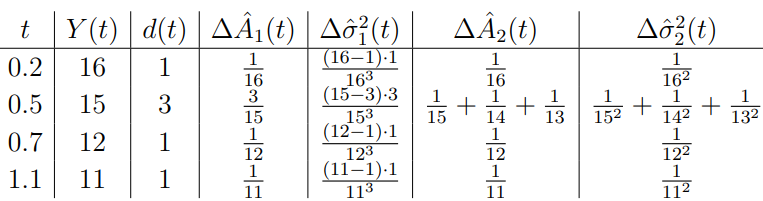
\includegraphics[width=10cm]{surv_table.png}

\medskip

\textbf{Example Population Hazard Rate}

Let $\alpha(t|Z) = \alpha(t)Z$ where $\mathcal{L}_Z(s) = \mathbb{E}[\text{exp}\{-sZ\}] = (1+\delta s)^{-1/\delta}$. We get that $\mathcal{L}'(s)\big|_{s=0}  = -\mathbb{E}[Z] = -\frac{\mathcal{L}_Z(s)}{1+\delta }\big|_{s=0} = -1 \implies \mathbb{E}[Z] = 1$ by derivating both sides with regards to $s$. We can obtain the population hazard rate $\mu(t) = \alpha(t)\frac{-\mathcal{L}_Z'(A(t))}{\mathcal{L}_Z(A(t))} = \frac{\alpha(t)}{1 + \delta A(t)}$. By assuming some form of $\alpha(t)$ (or $A(t)$) we can then examine the population hazard rate as $t \to \infty$. 

\medskip

\textbf{Example of Likelihood Derivations} We have $(i, t_i, \delta_i) = \left\{(1,1.23,1),(2,1.97,1),(3, 1.17, 0)\right\}$. If we assume that the times are $\text{Exp}(\nu)$ then we get $L(\nu; t_1, t_2, t_3) = \nu^2 e^{-\nu(t_1 + t_2)} e^{-t_3}$. 

\medskip

\textbf{Example of LR-test using Cox partial likelihood}
We have $\alpha(t; x) = \alpha_0(t)e^{\beta x}$ and 
$\{(T_i, \delta_i, x_i)\}_{i=1...5} = \{(1, 1, 1),(3, 1, 0),(4, 0, 1),(7, 0, 0),(10, 1, 1) \}$ then $L(\beta) = \frac{e^{\beta}}{e^{\beta}+1+e^{\beta}+1+e^{\beta}} \cdot \frac{1}{1+e^{\beta}+1+e^{\beta}} \cdot \frac{e^{\beta}}{e^{\beta}}$. We then perform the likelihood ratio test as described under \textbf{Testing} using $\hat\beta$ (which we obtain using regular likelihood theory) and $\beta_0$. 

\section*{Misc}

\textbf{Accelerated failure time models:} $\log U_i = \mathbf{\beta}^T\mathbf{x}_i + \varepsilon_i$ where $E[\varepsilon_i]=0$ iid. $\implies S_{U_i}(u)=P(U_i>u)=P(e^{\mathbf{\beta}^T\mathbf{x}_i + \varepsilon_i}>u) = \\ P(\underbrace{\mathbf{\varepsilon_i}}_{w_i} > ue^{-\mathbf{\beta}^T\mathbf{x}_i} = S_{w_i}(ue^{-\mathbf{\beta}^T\mathbf{x}_i})$, (change of time), $\implies S_{U_i}'(u) = S_{w_i}'(ue^{-\mathbf{\beta}^T\mathbf{x}_i})e^{-\mathbf{\beta}^T\mathbf{x}_i} \implies \alpha_{U_i}(u) = \frac{-S_{U_i}'(u)}{S_{U_i}(u)} = \alpha_{w_i}(ue^{-\mathbf{\beta}^T\mathbf{x}_i})ue^{-\mathbf{\beta}^T\mathbf{x}_i}$

\medskip

\textbf{Likelihood} With censored observations we can express the likelihood as follows. $L(\theta; t_1,...,t_n)\prod_{i=1}^n \mathbb{P}(T = t_i)^\delta_i \mathbb{P}(T \geq t_i)^{1-\delta_i}$ where $\delta_i$ is the indicator of $t_i$ being censored. See example below under \textbf{Examples}

\medskip

\textbf{Likelihood in terms of hazard rate} $L(\theta) = \prod_{i\in \mathcal{D}_i}\mathbb{P}(T\in[t_i, t_i +dt;\theta))\prod_{i\notin \mathcal{D}_i}\mathbb{P}(T\geq t_i; \theta) \approx \prod_{i \in \mathcal{D}_i} f(t_i;\theta)dt\prod_{i \notin \mathcal{D}} S(t_i; \theta)$ \newline $\propto \prod_{i\in \mathcal{D}_i}\alpha(t_i;\theta)S(t_i;\theta)\prod_{i\notin \mathcal{D}_i}S(t_i;\theta) = \prod_{i=1}^n \alpha(t_i,\theta)^{\delta_i}S(t_i;\theta)$ where individuals with $\delta_i = 1$ belong to $\mathcal{D}_i$.

\medskip

\end{document}
